%%%%%%%%%%%%%%%%%%%%%%%%%%%%%%%%%%%%%%%%%
% Beamer Presentation - MIWAI 2026 (Paper 122, oral)
% Two-Branch Hybrid Model for Imbalanced Lumbar Disc Grading
% Template: Madrid + HCMUT institute (follows thesis-defense deck style)
%%%%%%%%%%%%%%%%%%%%%%%%%%%%%%%%%%%%%%%%%

\documentclass{beamer}

\mode<presentation> {
\usetheme{Madrid}
}

\usepackage[utf8]{inputenc}
\usepackage[T1]{fontenc}
\usepackage{graphicx}
\usepackage{booktabs}
\usepackage{multirow}
\usepackage{amsmath}
\usepackage{amssymb}
\usepackage{tikz}
\usetikzlibrary{positioning,arrows.meta,fit,backgrounds,calc}

\usepackage[sorting=none,backend=biber]{biblatex}
\addbibresource{references.bib}
\addbibresource{slides_extra.bib}
% Bibliography entries stay small so the references slide fits.
\setbeamerfont{bibliography item}{size=\scriptsize}
\setbeamerfont{bibliography entry author}{size=\scriptsize}
\setbeamerfont{bibliography entry title}{size=\scriptsize}
\setbeamerfont{bibliography entry location}{size=\scriptsize}
\setbeamerfont{bibliography entry note}{size=\scriptsize}
\setbeamertemplate{bibliography item}[text]

\graphicspath{{figures/}}

% Best-cell highlight (matches the paper)
\definecolor{best}{HTML}{1A4DAB}
\newcommand{\bst}[1]{\textcolor{best}{\textbf{#1}}}

% Custom three-part footline (same layout as the thesis-defense deck)
\setbeamertemplate{footline}
{%
  \leavevmode%
  \hbox{%
  \begin{beamercolorbox}[wd=.333333\paperwidth,ht=2.25ex,dp=1ex,center]{author in head/foot}%
    \usebeamerfont{title in head/foot}\insertshorttitle
  \end{beamercolorbox}%
  \begin{beamercolorbox}[wd=.333333\paperwidth,ht=2.25ex,dp=1ex,center]{title in head/foot}%
    \usebeamerfont{title in head/foot}\insertsectionhead
  \end{beamercolorbox}%
  \begin{beamercolorbox}[wd=.333333\paperwidth,ht=2.25ex,dp=1ex,leftskip=2ex,rightskip=2ex,sep=0pt]{date in head/foot}%
    \hfill%
    \usebeamerfont{date in head/foot}\insertshortdate{}\hfill%
    \usebeamercolor[fg]{page number in head/foot}%
    \usebeamerfont{page number in head/foot}%
    \usebeamertemplate{page number in head/foot}%
  \end{beamercolorbox}}%
  \vskip0pt%
}
\setbeamertemplate{caption}[numbered]

%----------------------------------------------------------------------------------------
%	TITLE PAGE
%----------------------------------------------------------------------------------------
\title[Two-Branch Hybrid Grading]{A Two-Branch Hybrid Model for Imbalanced Lumbar Disc Grading and Zero-Shot Label Extension}

\author[T.\,K.~Ha, T.\,N.~Phan]{Trung Kien Ha \and Trong Nhan Phan}
\institute[HCMUT, VNU-HCM]
{
Faculty of Computer Science and Engineering \\
Ho Chi Minh City University of Technology (HCMUT), VNU-HCM \\
\medskip
\textit{MIWAI 2026, Paper 122}
}
\date{October 2026}

\begin{document}

\begin{frame}
\titlepage
\end{frame}

\begin{frame}
\frametitle{Outline}
\tableofcontents
\end{frame}

%----------------------------------------------------------------------------------------
\section{Motivation}
%----------------------------------------------------------------------------------------
\begin{frame}
\frametitle{Two open problems in lumbar MRI grading}
\begin{columns}[c]
\column{.42\textwidth}
\begin{itemize}
    \item[\textbf{P1}] \textbf{Class imbalance} \\ {\small Severe $<5\%$ $\Rightarrow$ recall near zero}
    \item[]
    \item[\textbf{P2}] \textbf{Fixed label space} \\ {\small new schema $\Rightarrow$ retrain a new head}
\end{itemize}
\vspace{4pt}
{\scriptsize Today a radiologist grades each disc by hand, and different readers often disagree on the grade~\cite{nigru2024}.}
\column{.58\textwidth}
\centering
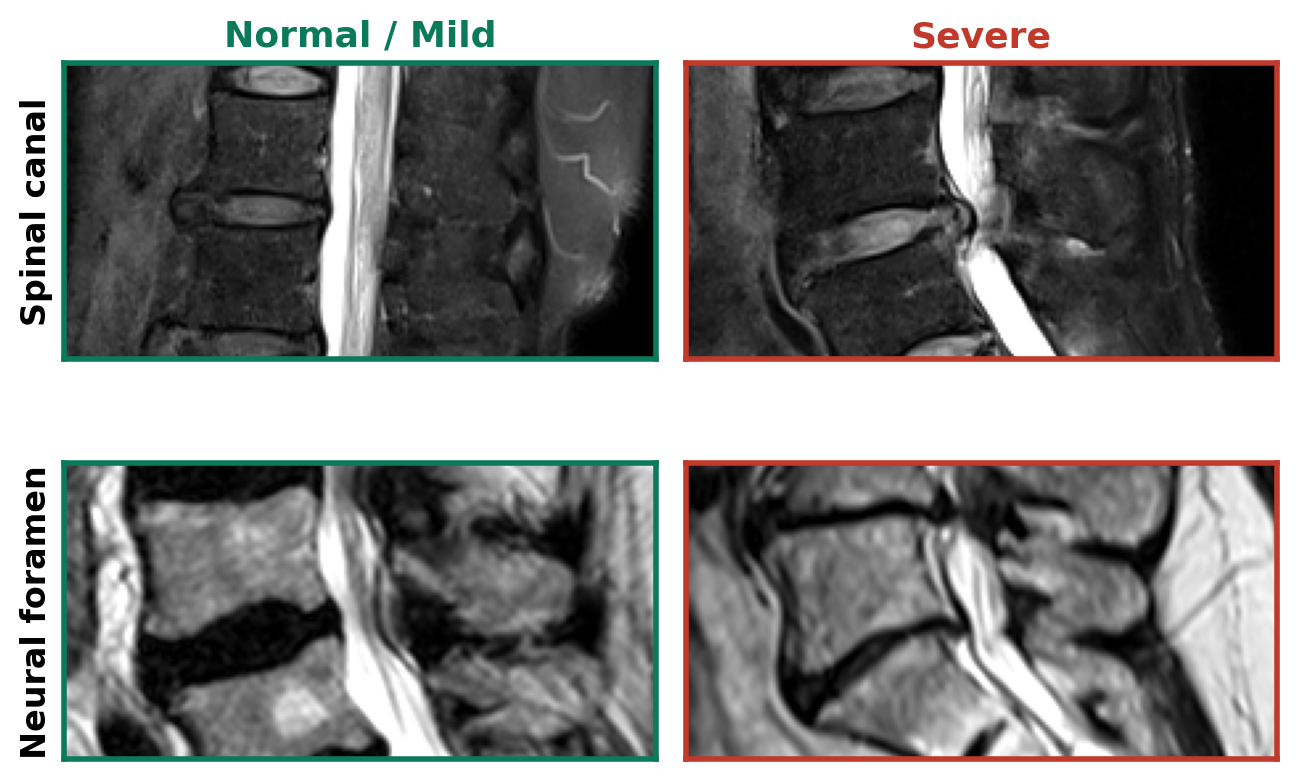
\includegraphics[width=\linewidth]{abnormality_examples_en.png}\\[2pt]
{\scriptsize Sagittal T2/STIR crops, RSNA 2024~\cite{kaggle2024}: the Severe cases we keep missing.}
\end{columns}
\end{frame}

\begin{frame}
\frametitle{Contributions}
\begin{enumerate}
    \item Attention helps Severe \textbf{in-domain} but hurts \textbf{transfer}; frozen prior recovers it to parity.
    \item Complementary \textbf{two-branch} design (attention + biomedical VLM).
    \item \textbf{Zero-shot} label extension: swap the prompts, no new head, no retraining.
    \item Imbalance recipe lifts Severe recall \textbf{12.3\% $\to$ 48.6\%} ($\sim$4$\times$).
\end{enumerate}
\end{frame}

%----------------------------------------------------------------------------------------
\section{Proposed Method}
%----------------------------------------------------------------------------------------
\begin{frame}
\frametitle{Two-branch hybrid architecture}
\begin{figure}
    \centering
    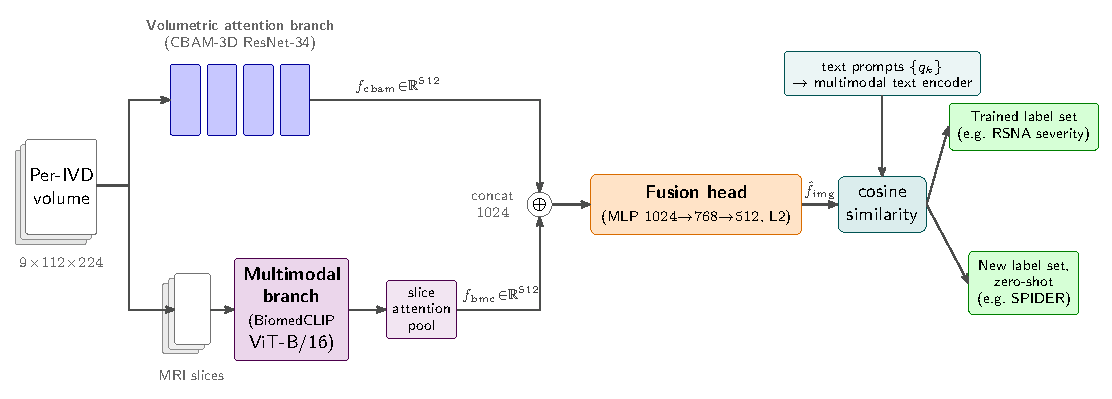
\includegraphics[width=\textwidth]{hybrid_arch_generic.pdf}
\end{figure}
\vspace{2pt}
\begin{itemize}\small
    \item[--] \textbf{Attention:} CBAM~\cite{woo2018cbam} 3D ResNet-34~\cite{windsor2022}: localizes the lesion.
    \item[--] \textbf{Multimodal:} frozen BiomedCLIP~\cite{zhang2023biomedclip}: text-aligned prior.
    \item[--] Fusion MLP $\to$ cosine similarity against the prompts.
\end{itemize}
\end{frame}

\begin{frame}
\frametitle{Handling class imbalance}
\begin{columns}[c]
\column{.52\textwidth}
\begin{itemize}\small
    \item[\textbf{1.}] \textbf{Focal loss}~\cite{lin2017focal}: let the hard cases drive the loss, not the many easy Normal ones.
    \item[\textbf{2.}] \textbf{Square-root class weights}: raise the rare class's gradient, without the instability of full inverse weighting.
    \item[\textbf{3.}] \textbf{Minority oversampling}~\cite{buda2018imbalance}: show Severe volumes more often in each epoch.
    \item[\textbf{4.}] \textbf{Augmentation}~\cite{shorten2019augmentation}: get more variation out of the few Severe volumes there are.
\end{itemize}
\column{.48\textwidth}
\centering
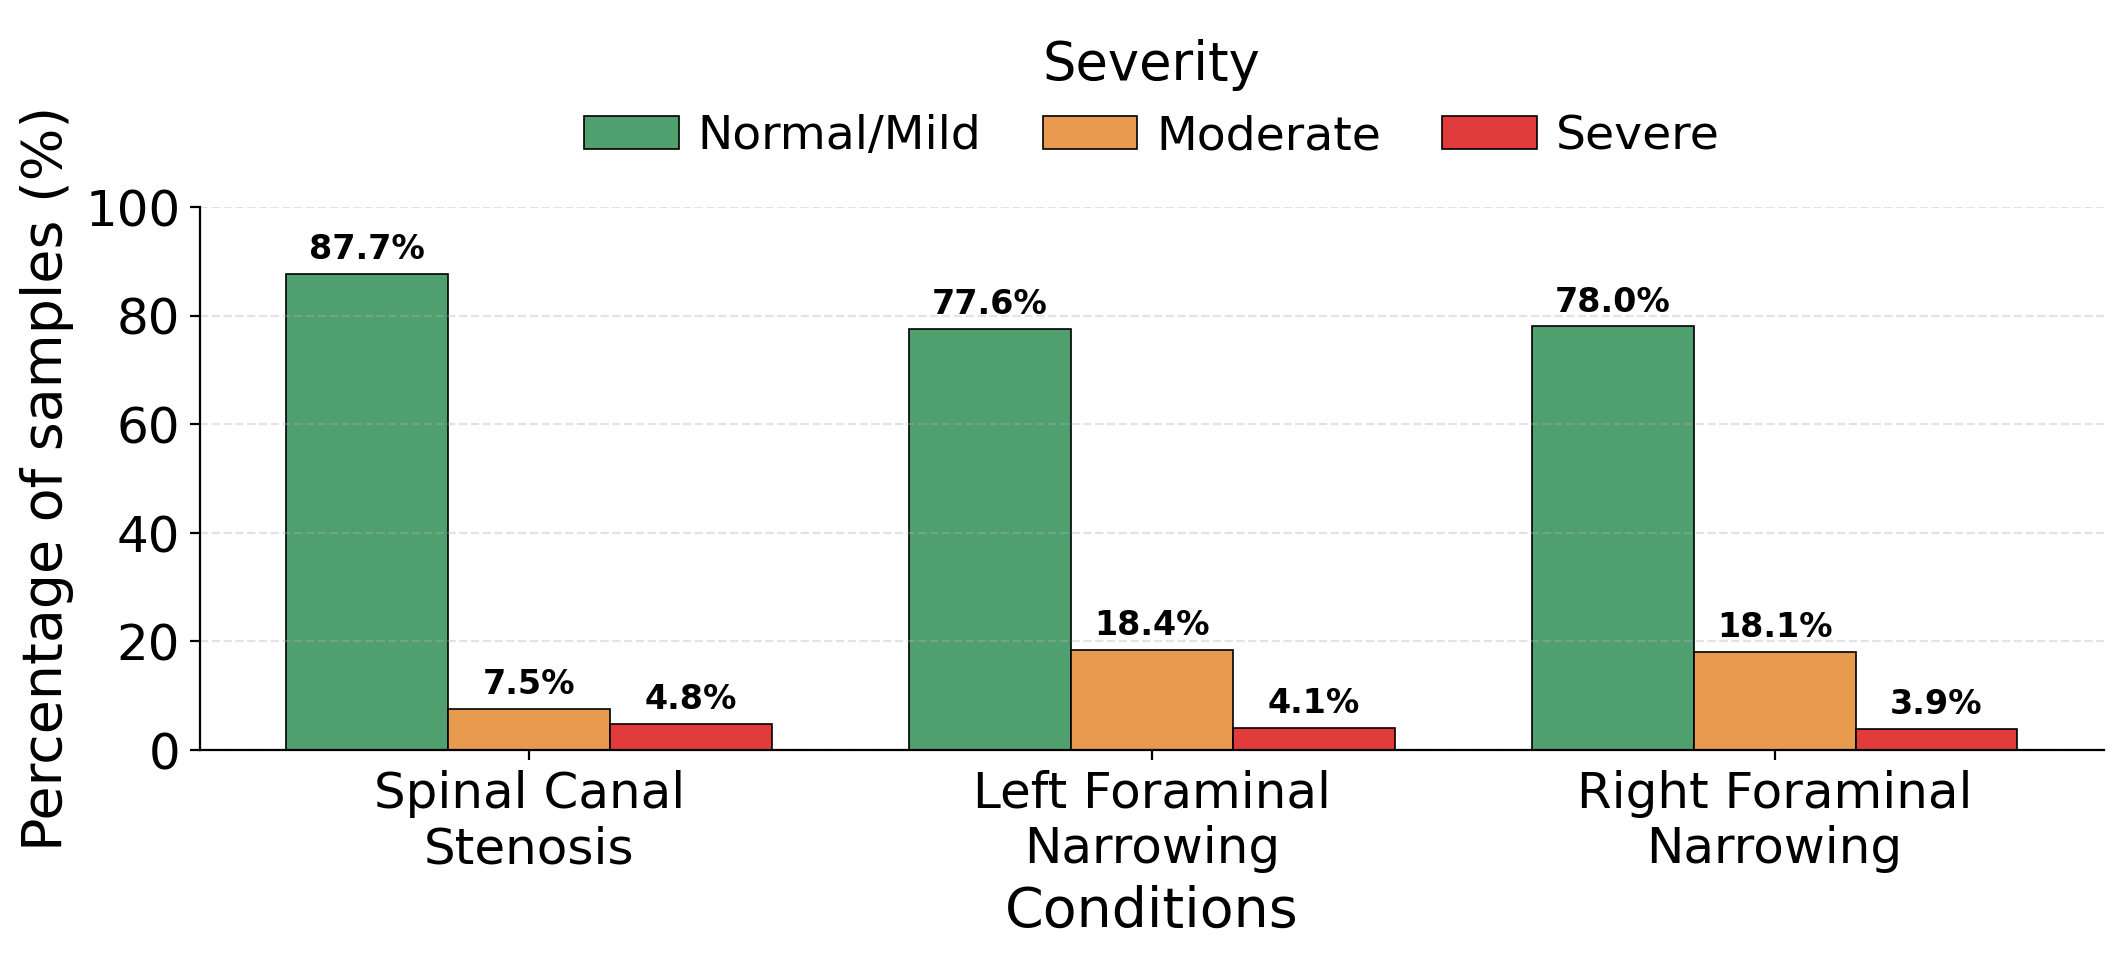
\includegraphics[width=\linewidth]{rsna_class_distribution_en.png}\\[2pt]
{\scriptsize RSNA 2024: Severe is the smallest class in all three conditions.}
\end{columns}
\end{frame}

\begin{frame}
\frametitle{Zero-shot label extension by prompts}
Same encoder $\Phi$, only the head changes ($h = c \circ \Phi$):
\begin{equation*}
\hat{y} = \arg\max_{k}\; s\cdot \hat{f}_{\text{img}}^{\top}\, t_k ,
\qquad t_k = \psi(q_k)/\|\psi(q_k)\|_2 .
\end{equation*}
\begin{itemize}\small
    \item[--] Every class is written as a phrase $q_k$; the frozen text encoder $\psi$
          turns it into an anchor $t_k$ (e.g.\ \textit{``severe spinal canal stenosis''}).
    \item[--] Anchors are encoded \textbf{once} and reused. The volume is the only
          per-case input, and $\{t_k\}$ sits where a weight matrix would.
    \item[--] A different label schema is a different set of phrases.
    \item[$\Rightarrow$] New label = new prompt. \textbf{No new head, no retraining.}
\end{itemize}
\end{frame}

%----------------------------------------------------------------------------------------
\section{Experiments}
%----------------------------------------------------------------------------------------
\begin{frame}
\frametitle{Experimental setup: data}
\begin{columns}[c]
\column{.5\textwidth}
{\footnotesize
\begin{tabular}{@{}ll@{}}
\toprule
\multicolumn{2}{@{}l}{\textbf{RSNA 2024}~\cite{kaggle2024}} \\
\midrule
Validation & 1{,}942 IVDs / 395 pts \\
Sequence   & sagittal T2 / STIR \\
Labels     & 3 conditions $\times$ 3 severities \\
Role       & train + in-domain test \\
\midrule
\multicolumn{2}{@{}l}{\textbf{SPIDER}~\cite{vandergraaf2024spider}} \\
\midrule
Validation & 1{,}439 IVDs / 208 pts \\
Labels     & 8 disease labels \\
Role       & held-out transfer only \\
\bottomrule
\end{tabular}}
\vspace{5pt}

{\scriptsize One volumetric crop per disc, L1--L2 to L5--S1; intensities clipped to the 1st--99th percentile and rescaled to $[0,1]$.}
\column{.5\textwidth}
\centering
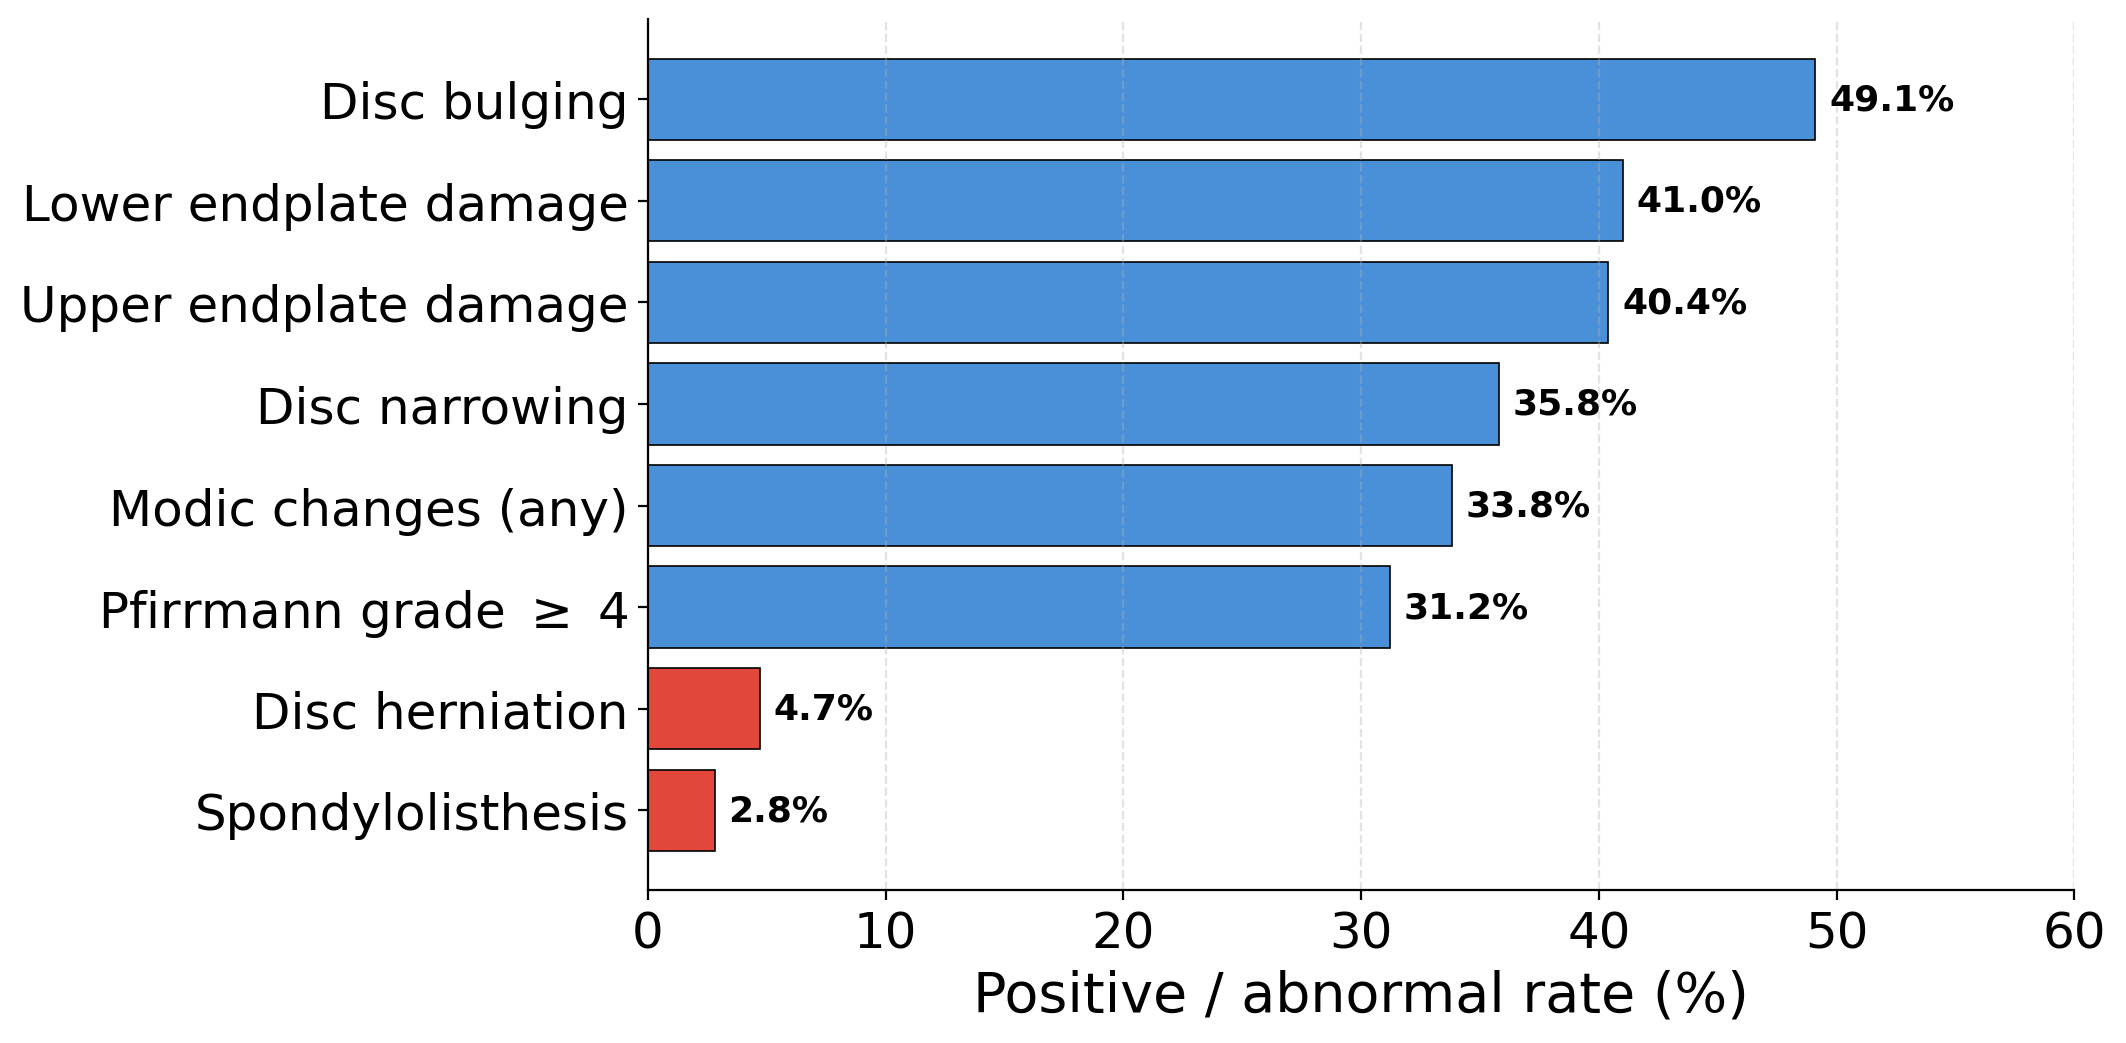
\includegraphics[width=\linewidth]{spider_class_distribution_en.png}\\[2pt]
{\scriptsize SPIDER: several labels are heavily skewed too.}
\end{columns}
\end{frame}

\begin{frame}
\frametitle{Experimental setup: training and protocol}
\begin{table}
\centering
\footnotesize
\renewcommand{\arraystretch}{1.15}
\begin{tabular}{@{}l p{6.1cm}@{}}
\toprule
\textbf{Setting} & \textbf{Value} \\
\midrule
Per-IVD input & $1\times9\times112\times224$; embedding dim $d=512$ \\
Trainable / total & 1.18\,M / 260\,M (both backbones frozen) \\
Optimizer & AdamW, lr $10^{-4}$, weight decay $10^{-4}$ \\
Batch / epochs & 32 / $\leq$20, early stopping (patience 5) \\
Augmentation & h-flip + L/R swap, rotate $\pm10^{\circ}$, bright./contrast $\pm20\%$, noise $\sigma{=}0.05$ ($p{=}0.3$) \\
Hardware & 1$\times$ RTX 4090 ($\approx$16\,GB peak) \\
\bottomrule
\end{tabular}
\end{table}
\vspace{2pt}
\begin{itemize}\small
    \item[--] 4 configs: SpineNetV2~\cite{windsor2022} / CBAM / Multimodal / \textbf{Hybrid}.
    \item[--] Macro Recall, Precision, F1, AUC (OvR), AUPRC, plus per-class Severe.
    \item[--] 3 seeds $\{42, 123, 456\}$; we report mean $\pm$ std.
\end{itemize}
\end{frame}

\begin{frame}
\frametitle{In-domain results \& ablation on RSNA 2024}
\begin{table}
\centering
\scriptsize
\setlength{\tabcolsep}{3pt}
\renewcommand{\arraystretch}{1.05}
\begin{tabular}{lcccc}
\toprule
\textbf{Metric} & \textbf{SpineNetV2} & \textbf{CBAM-only} & \textbf{Multimodal-only} & \textbf{Hybrid (Ours)} \\
\midrule
Mean Accuracy        & \bst{81.0} & 69.5 & 71.2 & 72.4 \\
Mean F1 (macro)      & 0.420 & 0.477 & 0.482 & \bst{0.527} \\
Mean Recall          & 0.412 & 0.531 & 0.532 & \bst{0.592} \\
Mean AUC             & 0.835 & 0.803 & 0.826 & \bst{0.838} \\
Mean AUPRC           & 0.530 & 0.498 & 0.513 & \bst{0.533} \\
\midrule
\textbf{Severe Recall} & 0.123 & 0.288 & 0.316 & \bst{0.486} \\
\textbf{Severe F1}   & 0.152 & 0.262 & 0.268 & \bst{0.356} \\
\textbf{Severe AUC}  & 0.872 & 0.865 & 0.885 & \bst{0.899} \\
\bottomrule
\end{tabular}
\caption{RSNA 2024 validation, mean over 3 seeds. \bst{Bold} = best. ``SpineNetV2'' is its grading backbone retrained here, not the published pipeline.}
\end{table}
\end{frame}

\begin{frame}
\frametitle{Putting the Severe metrics in context}
\begin{columns}[c]
\column{.5\textwidth}
\begin{itemize}
    \item[--] Severe prevalence $\approx$\textbf{0.05}.
    \item[--] Severe \textbf{AUC 0.899}, \textbf{AUPRC 0.333} = \textbf{6.7$\times$} chance.
    \item[--] Grad-CAM~\cite{selvaraju2017gradcam}: diffuse without attention; with CBAM it concentrates on the narrowed canal.
\end{itemize}
\column{.5\textwidth}
\centering

\includegraphics[width=\linewidth]{grad_cam_nocbam_vs_cbam.png}\\[2pt]
{\scriptsize Severe canal case: without vs.\ with CBAM.}
\end{columns}
\end{frame}

\begin{frame}
\frametitle{Cross-dataset zero-shot transfer to SPIDER}
\centering
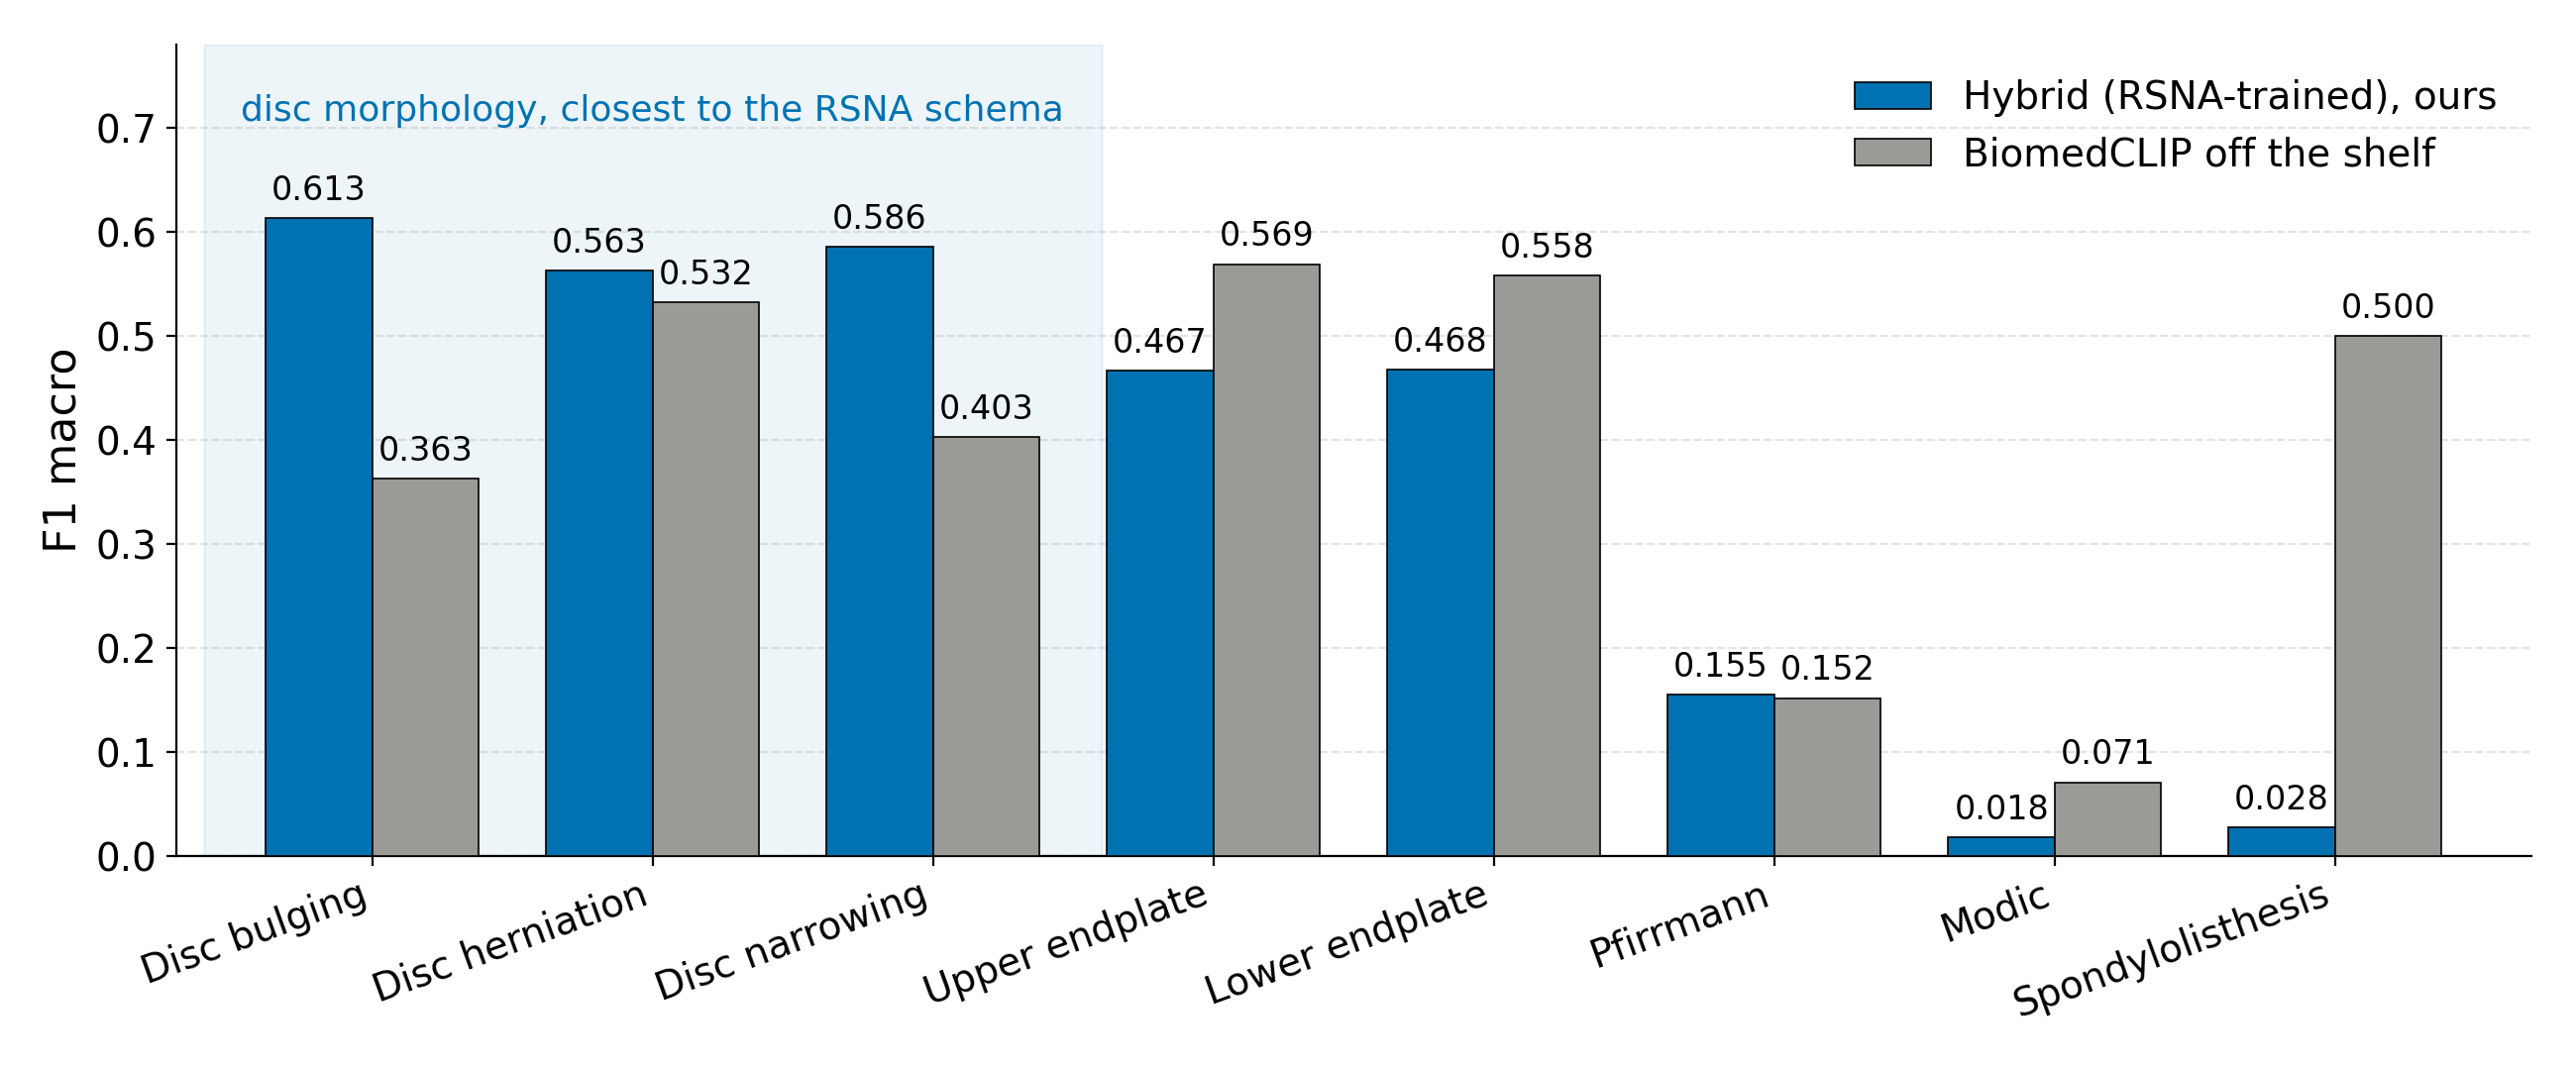
\includegraphics[width=.95\textwidth]{spider_zeroshot_en.png}
\vspace{1pt}
\begin{itemize}\scriptsize
    \item[--] 8 \textbf{unseen} labels, no SPIDER training: only new prompts. Wins on disc morphology (\bst{0.587} vs.\ 0.433), loses on distant labels (all-8: \bst{0.394} off the shelf vs.\ 0.362 ours).
\end{itemize}
\end{frame}

\begin{frame}
\frametitle{Supervised transfer on SPIDER (8 labels)}
\begin{table}
\centering
\footnotesize
\renewcommand{\arraystretch}{1.15}
\begin{tabular}{lcccc}
\toprule
\textbf{Metric} & \textbf{SpineNetV2} & \textbf{CBAM-only} & \textbf{Multimodal-only} & \textbf{Hybrid (Ours)} \\
\midrule
Mean Accuracy (\%) & \bst{80.2} & 79.3 & 76.1 & 78.3 \\
Mean F1 (macro)    & 0.646 & 0.619 & 0.613 & \bst{0.653} \\
Mean AUC           & 0.842 & 0.824 & 0.808 & \bst{0.846} \\
Mean AUPRC         & \bst{0.633} & 0.580 & 0.544 & 0.611 \\
\bottomrule
\end{tabular}
\end{table}
\begin{itemize}\small
    \item[--] Hybrid and SpineNetV2 are at \textbf{parity}. We do not claim to surpass it.
    \item[--] CBAM alone \textbf{falls below} plain SpineNetV2 on transfer: 0.619 against 0.646.
    \item[--] The hybrid \textbf{recovers} to 0.653, above CBAM by $+0.034$.
    \item[$\Rightarrow$] The frozen branch acts as a \textbf{regularizer} on transfer.
    \item[--] {\footnotesize Three seeds, so the $p$-values are exploratory, not a powered test.}
\end{itemize}
\end{frame}

%----------------------------------------------------------------------------------------
\section{Conclusion}
%----------------------------------------------------------------------------------------
\begin{frame}
\frametitle{Take-aways}
\begin{itemize}
    \item[\textbf{1.}] Recovers Severe class: Recall $\times 4$, F1 $\times 2.3$, AUC 0.899.
    \item[\textbf{2.}] \textbf{Zero-shot} to 8 unseen labels, no retraining.
    \item[\textbf{3.}] Frozen branch = \textbf{cross-dataset regularizer}.
\end{itemize}
\vspace{6pt}
\begin{block}{Future work}
\begin{itemize}\small
    \item[--] An explicit image-text alignment loss.
    \item[--] A native 3D medical vision-language backbone.
    \item[--] Axial T2 alongside sagittal, for the foraminal conditions.
\end{itemize}
\end{block}
\vspace{4pt}
{\footnotesize Clinical use: second-reader assistant (Severe recall still below screening bar).}
\end{frame}

%------------------------------------------------
\begin{frame}
\centering
\vfill
{\Huge Thank you}\\[14pt]
{\LARGE Questions?}
\vfill
{\footnotesize Trung Kien Ha \, $\cdot$ \, Trong Nhan Phan \quad$\cdot$\quad HCMUT, VNU-HCM}
\vfill
\end{frame}

%------------------------------------------------
\begin{frame}[allowframebreaks]
\frametitle{References}
\printbibliography[heading=none]
\end{frame}

%------------------------------------------------
% BACKUP SLIDES
%------------------------------------------------
\appendix
\begin{frame}
\frametitle{Backup: full RSNA metrics}
\begin{table}
\centering
\scriptsize
\setlength{\tabcolsep}{3pt}
\begin{tabular}{lcccc}
\toprule
\textbf{Metric} & \textbf{SpineNetV2} & \textbf{CBAM-only} & \textbf{Multimodal-only} & \textbf{Hybrid (Ours)} \\
\midrule
Mean Precision  & 0.493 & 0.499 & 0.508 & \bst{0.526} \\
Severe AUPRC    & 0.284 & 0.278 & 0.275 & \bst{0.333} \\
Inference (ms/IVD)$^{\dagger}$ & 65.5 & 66.7 & 65.2 & 66.4 \\
\bottomrule
\end{tabular}
\end{table}
{\scriptsize $^{\dagger}$Timing is measured on the SPIDER transfer run, not on RSNA.}
\end{frame}

\begin{frame}
\frametitle{Backup: per-label zero-shot on SPIDER}
\begin{table}
\centering
\scriptsize
\setlength{\tabcolsep}{4pt}
\begin{tabular}{lcc}
\toprule
\textbf{SPIDER label} & \textbf{Off-shelf BiomedCLIP} & \textbf{Hybrid} \\
\midrule
Disc bulging         & 0.363 & \bst{0.613} \\
Disc herniation      & 0.532 & \bst{0.563} \\
Disc narrowing       & 0.403 & \bst{0.586} \\
\midrule
Upper endplate       & \bst{0.569} & 0.467 \\
Lower endplate       & \bst{0.558} & 0.468 \\
Pfirrmann (5-class)  & 0.152 & \bst{0.155} \\
Spondylolisthesis    & \bst{0.500} & 0.028 \\
Modic (4-class)      & \bst{0.071} & 0.018 \\
\midrule
Mean (disc morphology) & 0.433 & \bst{0.587} \\
Mean (all 8)           & \bst{0.394} & 0.362 \\
\bottomrule
\end{tabular}
\end{table}
{\scriptsize Modic needs the paired T1 sequence SPIDER does not provide: a task-input limit, not a model one.}
\end{frame}

\begin{frame}
\frametitle{Backup: core equations}
\textbf{CBAM (3D):}\;
$F' = M_c(F)\otimes F,\quad F'' = M_s(F')\otimes F'$,\;
$F\in\mathbb{R}^{C\times D\times H\times W}$.\\[6pt]
\textbf{Focal loss} ($\gamma{=}2.0$ here; $1.8$ for CBAM-only):
$\;\mathrm{FL}_t(p_t) = -\,w_{c(t)}\,(1-p_t)^{\gamma}\,\log(p_t).$\\[6pt]
\textbf{Slice-attention pool:}
$\;\alpha_i = \dfrac{\exp(w_a^\top z_i)}{\sum_j \exp(w_a^\top z_j)},\quad
f_{\text{bmc}} = \sum_i \alpha_i z_i .$
\end{frame}

\begin{frame}
\frametitle{Backup: full training objective}
\begin{itemize}\small
    \item[--] No linear head. Logits = \textbf{cosine} vs.\ frozen text anchors:
      $\;s\cdot\hat f^\top t_k$, with $s$ a \textbf{learned} logit scale (clamp 100).
    \item[--] Focal loss ($\gamma{=}2.0$; $1.8$ for CBAM-only) applied \textbf{to those cosine logits}.
    \item[--] $+$ per-task \textbf{supervised contrastive} term~\cite{khosla2020supcon} ($\lambda{=}0.1$, $\tau{=}0.07$).
    \item[--] Tasks combined by learned \textbf{homoscedastic uncertainty} weighting~\cite{kendall2018multitask}, not a plain sum.
    \item[--] Missing labels ($-1$) excluded from both terms.
    \item[--] SpineNetV2 baseline uses plain \textbf{cross-entropy}; the other three use focal.
\end{itemize}
\end{frame}

\begin{frame}
\frametitle{Backup: parameters \& statistics}
\begin{itemize}\small
    \item[--] Both backbones stay frozen: the volumetric encoder and BiomedCLIP.
    \item[--] Trained: fusion MLP, slice-pool, logit scale, uncertainty scalars = \textbf{1.18\,M} (0.45\% of 260\,M).
    \item[--] Hybrid vs.\ CBAM: $\Delta{=}{+}0.034$, $p{=}0.011$, CI $[0.018,0.049]$.
    \item[--] Hybrid vs.\ SpineNetV2: parity, $p{=}0.57$. Exploratory (3 seeds).
\end{itemize}
\end{frame}

\end{document}
